
\section{Equations}\label{S_Eq}

\subsection{Pyrolysis Kinetic Equations}\label{SS_KinEq}
In PKP are four possible kinetic models to select:
\begin{itemize}
 \item The Constant Rate Model, section~\ref{SSS_cR}
 \item The Arrhenius Model, \ref{SSS_Arrh}
 \item The Kobayashi Model, \ref{SSS_Kob}
 \item The Distributed Activation Energy Model, \ref{SSS_DAEM}
\end{itemize}
The Kobayashi model has the advantage, that the yields are dependent on the individual temperature history. A change, may in in the final temperature leads to a higher yield.\\
The constant rate and the Arrhenius model has fixed final yields. The general devolatilization reactions for these two models are described with equations~\ref{E_Reaction_s}~and~\ref{E_Reaction_g}, where~\ref{E_Reaction_s} describes the mass loss of the solid~(index~\textit{s}) coal, equation~\ref{E_Reaction_g} the formation of the yields~(gaseous:\textit{g}, individual:\textit{i}).
\begin{align}
\label{E_Reaction_s}
 \frac{dm_{s}}{dt}&=-k_s \: \left( m_{s} - m_{s,final} \right)\\
\label{E_Reaction_g}
 \frac{dm_{g,i}}{dt}&=k_{g,i} \: \left(m_{g,i,final} - m_{g,i}\right)  
\end{align}
So when using more than one run, also the final yield is a parameter to fit. It will be located in between the final yields of the runs of the pyrolysis models.

In the following subsections, the plots showing the rates and yields were generated with \CPD and \FGDVC showing the yields and rates for different species. All are based on the same temperature profiles as shown in figure~\ref{F_Tt}.
\begin{figure}
\centering%\capstart
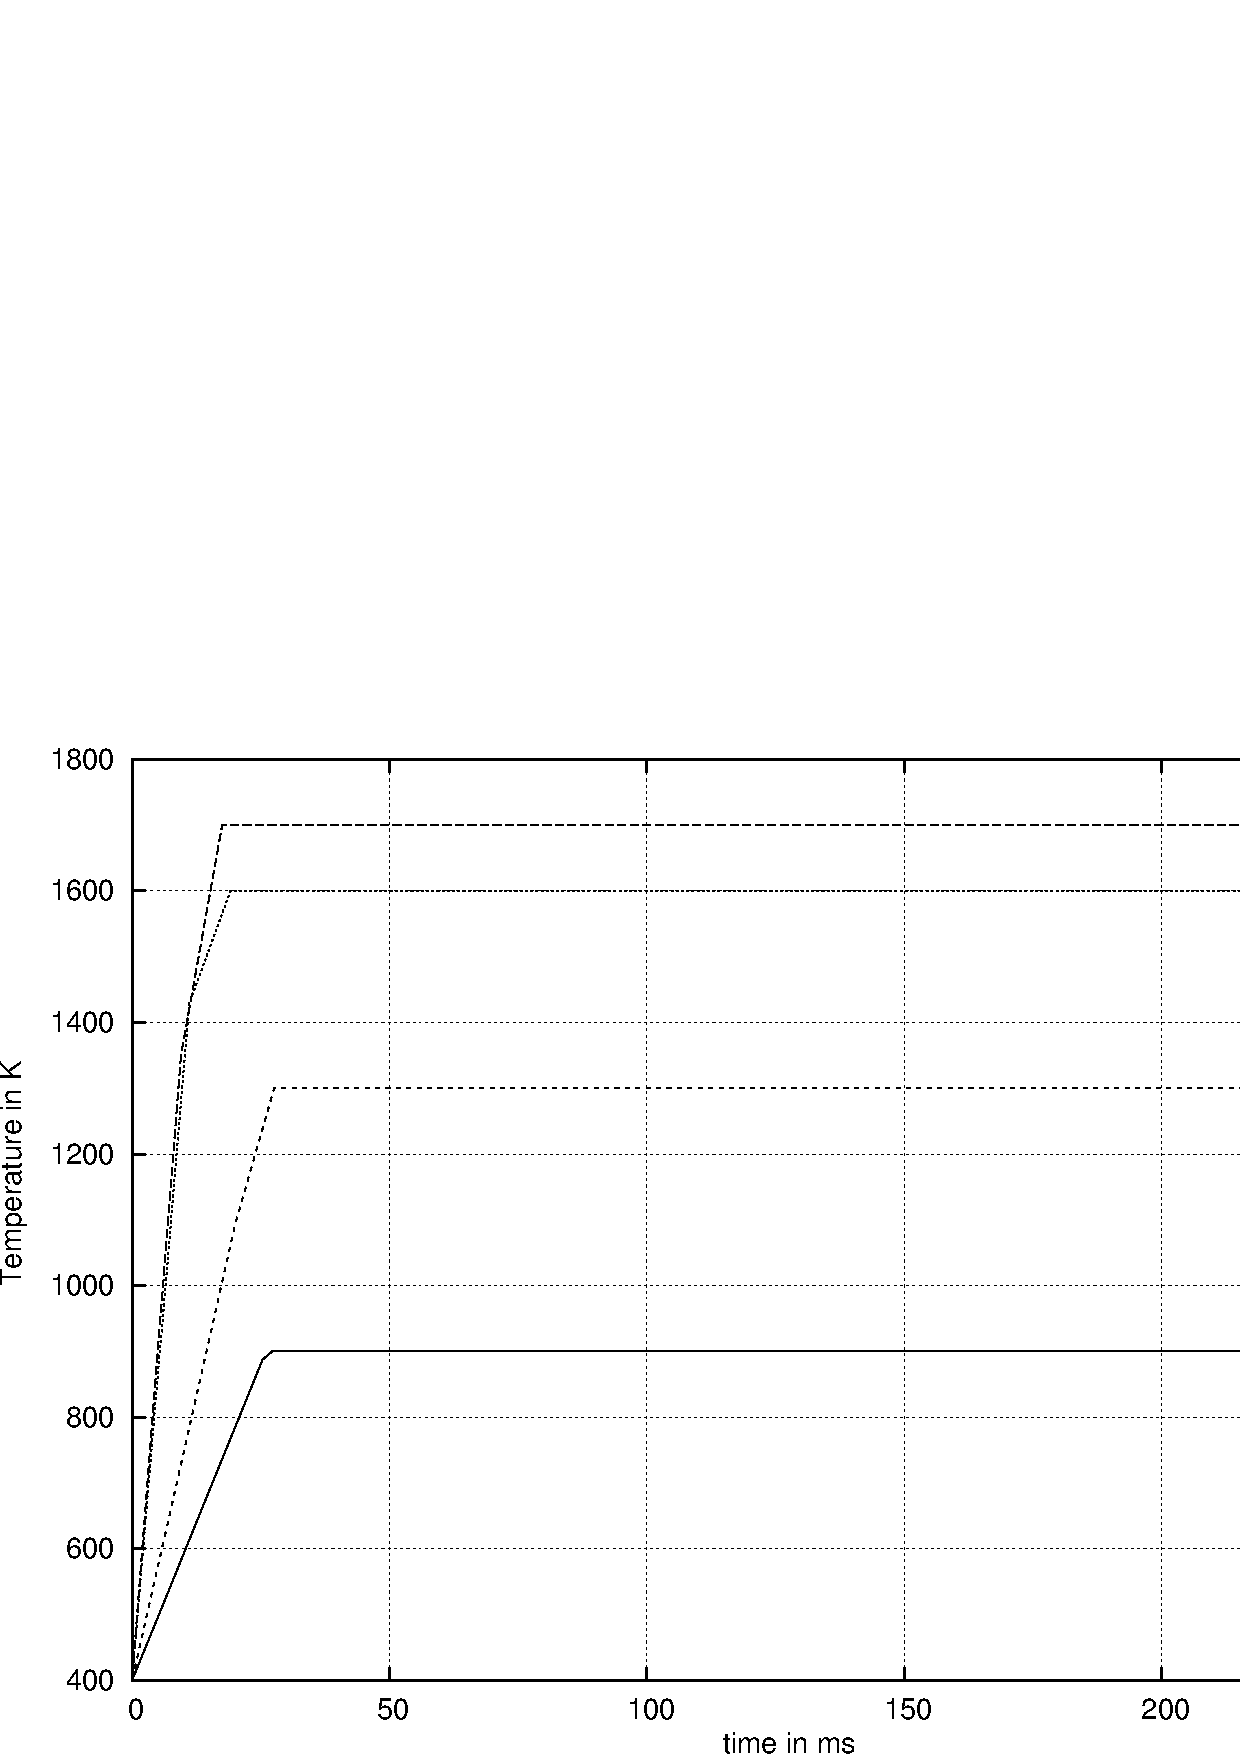
\includegraphics[height=8cm,angle=0]{Figures/tempHist}
\caption{The temperature history.}
\label{F_Tt}
\end{figure}

The table~\ref{T_Fit} gives an overview of the models with their parameters to fit and species to apply this model on. This is described more detailed in the next subsections.

\begin{table}
\newcommand{\mc}[3]{\multicolumn{#1}{#2}{#3}}
\begin{center}
\label{T_Fit}
\caption{The fitted models and their parameter.}
\begin{tabular}{lll}\hline
\textbf{Model} & \textbf{fitted parmeter} & \textbf{fitted species}\\\hline
constant Rate & \mc{1}{c}{$k_i$, $t_{start,i}$, $m_{final}$} & \mc{1}{c}{all}\\
Arrhenius & \mc{1}{c}{$A_i$, $b_i$, $E_i$, $m_{final}$} & \mc{1}{c}{all}\\
Kobyashi & \mc{1}{c}{$A_1$, $E_1$, $A_2$, $E_2$} & \mc{1}{c}{total}\\
DAEM & \mc{1}{c}{ } & \mc{1}{c}{ }\\\hline
\end{tabular}
\end{center}
\end{table}


\subsubsection{The Constant Rate Model}\label{SSS_cR}

Assuming a \textbf{constant rate} ($\mathrm{k = const. }$ and a starting time $\mathrm{t_{start}}$), the equations~\ref{E_Reaction_s}~and~\ref{E_Reaction_g} can be solved analytically:
\begin{align}
\label{E_constRate_s}
m_s(t)&=m_{s,final} + \left( m_{s}(t=t_{start,s}) - m_{s,final} \right) \: e^{-k_s(t-t_{start,s})}\\
\label{E_constRate_g}
m_{g,i}(t)&=m_{g,i,final}\cdot \left( 1 - \: e^{-k_i(t-t_{start,i})} \right)\\
\label{E_Offset_Time}
if \;\;\; t\leq t_i\::\;\;\; m(t)&=m(0)
\end{align}

This leads to advantage concerning the computational costs. On the other hand is this model completely independent from the temperature history. This is visualized in figure~\ref{F_Fit_cR_Y} where all fitted curves overlap each other.\\
The parameters to fit are for every species:
\begin{itemize}
 \item the starting time~($t_{start,i}$), where the devolatilization begins
 \item the constant rate factor $k_i$
 \item the final yield (when more than one run)
\end{itemize}
This model is applied to all species.

\begin{figure}
\centering%\capstart
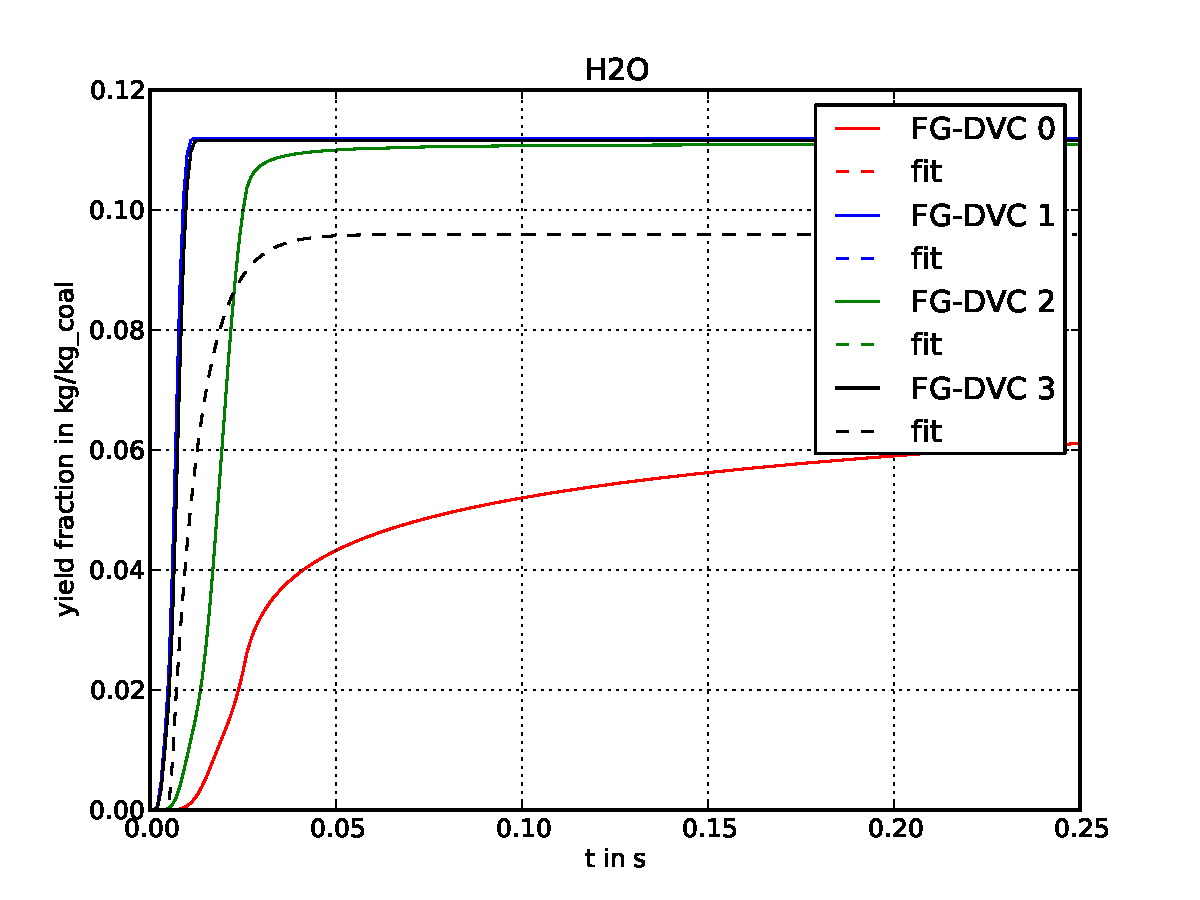
\includegraphics[height=9cm,angle=0]{Figures/FG-DVC-Fit_result_cR_H2O_Y}
\caption{One fitting result (Yields) for the constant Rate Model. The observed species is water.}
\label{F_Fit_cR_Y}
\end{figure}

%\begin{figure}
%\centering%\capstart
%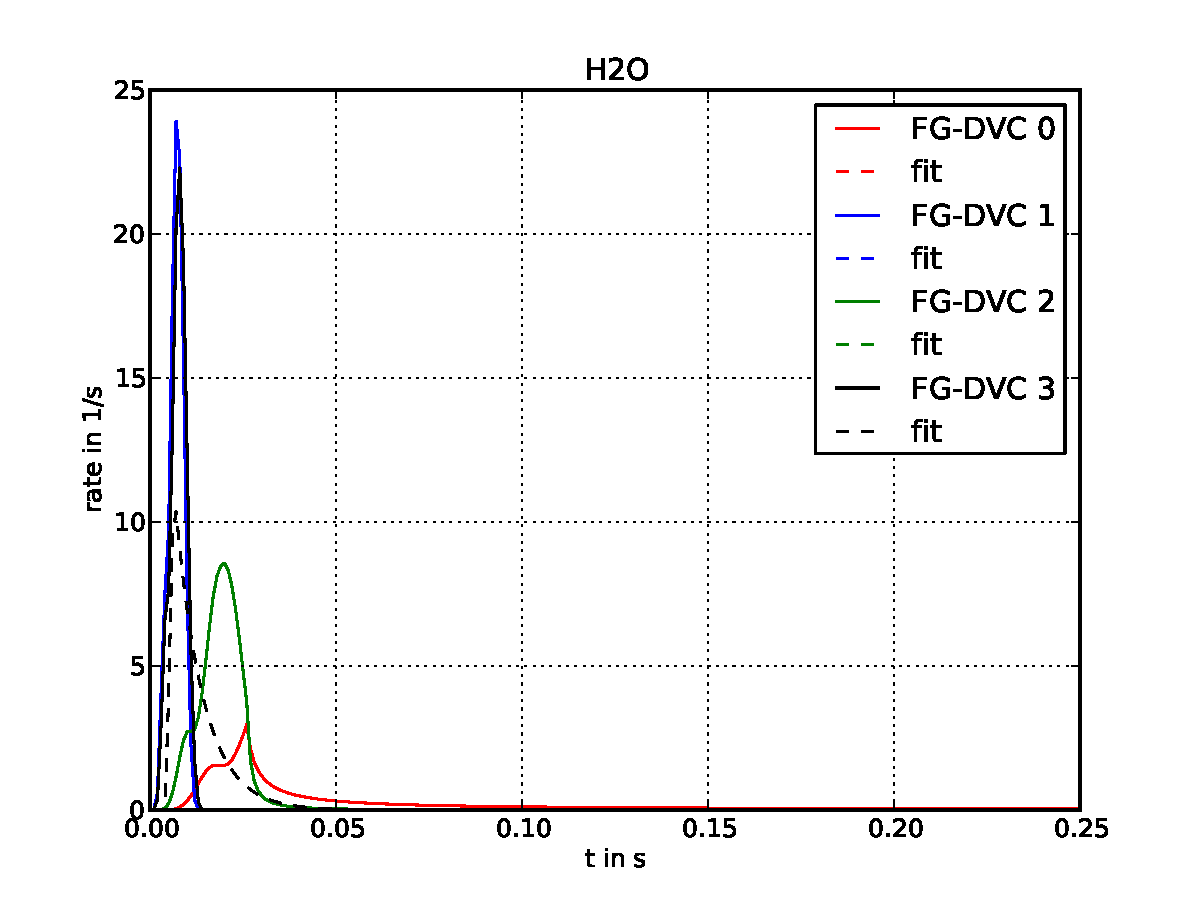
\includegraphics[height=9cm,angle=0]{Figures/FG-DVC-Fit_result_cR_H2O_R}
%\caption{One fitting result (Rates) for the constant Rate Model. The observed species is water.}
%\label{F_Fit_cR_R}
%\end{figure}

\subsubsection{The Arrhenius Model}\label{SSS_Arrh}

The kinetic rate k can be also expressed with the \textbf{Arrhenius} equation:
\begin{align}\label{E_Arrhenius_s}
 \frac{dm_s}{dt}&=A_s \cdot T(t)^{b_s} \cdot e^{-\frac{E_s}{T(t)}}\left( m_{s} - m_{s,final} \right)\\
\label{E_Arrhenius_g}
 \frac{dm_{g,i}}{dt}&=A_i \cdot T(t)^{b_{g,i}} \cdot e^{-\frac{E_{g,i}}{T(t)}}\left(m_{g,i,final} - m_{g,i}\right)
\end{align}
This notation of the Arrhenius equation includes no gas constant R in the exponential term. So the activation energy (or here more precise activation temperature) has the unit Kelvin. This is so far an advantage as the fitted $E_i$ is independent of the used unit system~(SI or cgs).\\
A second notation of the Arrhenius equation contains not the correction term $T(t)^{b_{g,i}}$:
\begin{align}\label{E_Arrhenius_s_noB}
 \frac{dm_s}{dt}&=A_s \cdot e^{-\frac{E_s}{T(t)}}\left( m_{s} - m_{s,final} \right)\\
\label{E_Arrhenius_g_noB}
 \frac{dm_{g,i}}{dt}&=A_i \cdot e^{-\frac{E_{g,i}}{T(t)}}\left(m_{g,i,final} - m_{g,i}\right)
\end{align}

Unlike the constant rate model is the Arrhenius modeled rate influenced by the temperature. But the Arrhenius model can be used to express the evolve for all species and the final yields are also fixed. So the parameter to fit are here:
\begin{itemize}
 \item the preexponentiation factor~$A_i$
 \item the correction factor $b_i$
 \item the activation energy $E_i$
 \item the final yield (when more than one run)
\end{itemize}
This model is applied to all species.\\

The Arrhenius model leads to a good agreement in the yield and rate curves for a limited range of temperatures, figures~\ref{F_Fit_Arrh_Y},~\ref{F_Fit_Arrh_R}. The disadvantage is the temperature independent yield fraction, all integrals for the rate curves in figure~\ref{F_Fit_Arrh_R} are the same. This leads to an imprecision as the yields show a dependency on the final temperature and heating rate.


\begin{figure}
\centering%\capstart
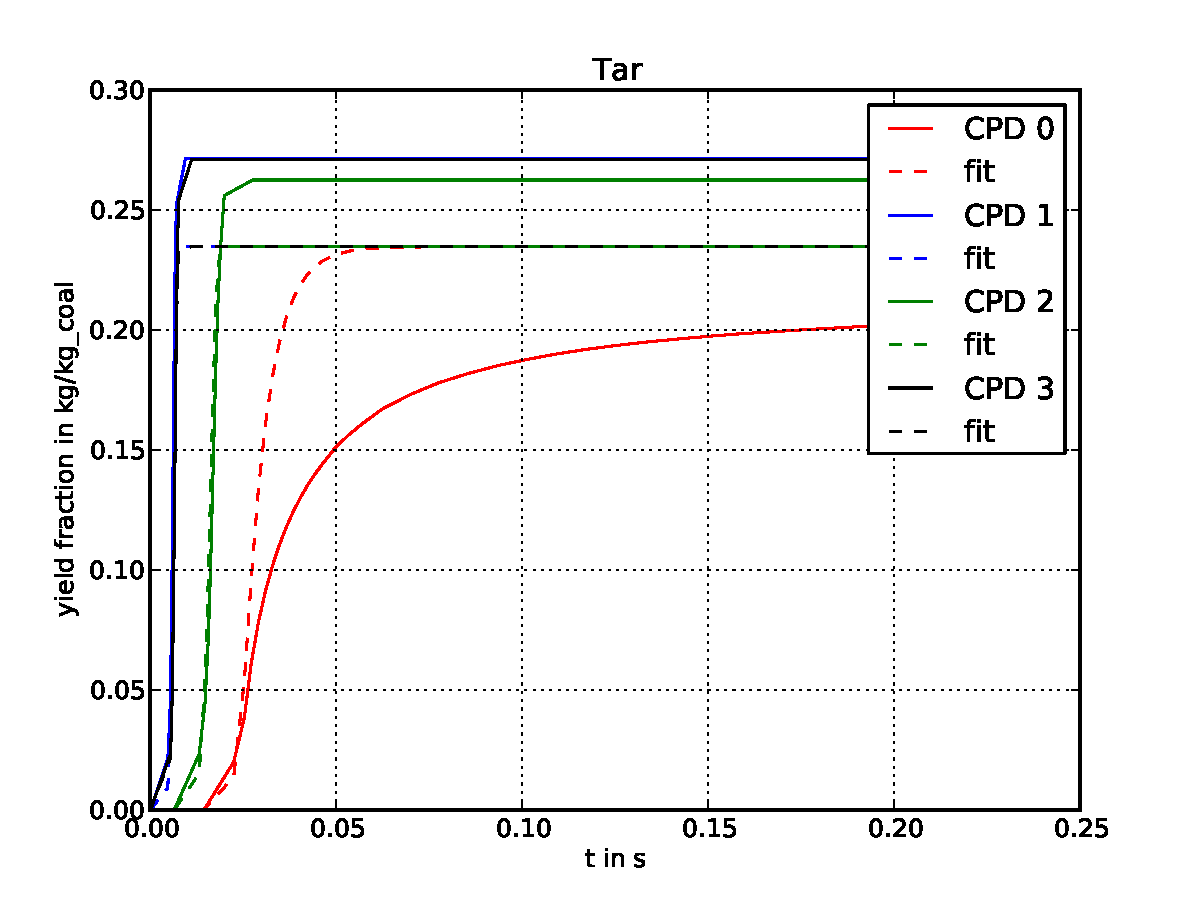
\includegraphics[height=9cm,angle=0]{Figures/CPD-Fit_result_Arrh_Tar_Y}
\caption{One fitting result (Yields) for the Arrhenius Model. The observed species is tar.}
\label{F_Fit_Arrh_Y}
\end{figure}

\begin{figure}
\centering%\capstart
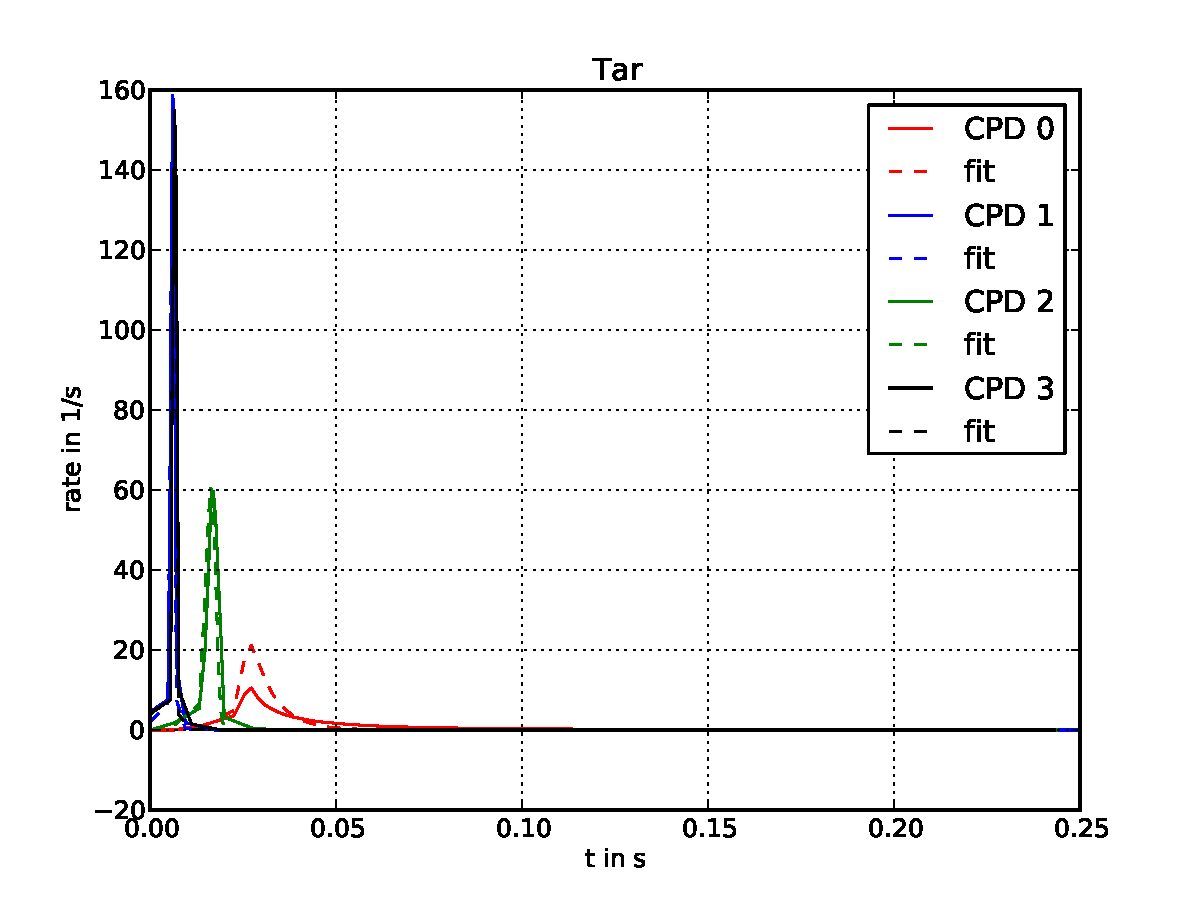
\includegraphics[height=9cm,angle=0]{Figures/CPD-Fit_result_Arrh_Tar_R}
\caption{One fitting result (Rates) for the Arrhenius Model. The observed species is tar.}
\label{F_Fit_Arrh_R}
\end{figure}

\subsubsection{The Kobayashi Model}\label{SSS_Kob}

Also the \textbf{Kobayashi} equation, also Two Competing Reaction Model, can be fitted, see equation~\ref{E_Kobayashi}. The optimization is carried out using the Arrhenius notation of equation~\ref{E_Kob_k} for $\mathrm{k_1}$ and $\mathrm{k_2}$.
\begin{equation}\label{E_Kobayashi}
 \frac{m_v(t)}{m_{p,0} - m_a}= \int_{0}^{t} ( \alpha_1 k_1 + \alpha_2 k_2 ) exp \left( -  \int_{0}^{t} ( k_1 + k_2 ) \; dt \right) \; dt
\end{equation}
\begin{equation}\label{E_Kob_k}
 k_j=A_j \:e^{-\frac{E_{j}}{T(t)}} \;\;\;\;\;\; with \: j=1,2
\end{equation}

The Kobayashi model can be applied only on the the overall, the total yields. The yield of individual species could be generated by multiplying the overall yield with the yield fraction~$\frac{y_i}{y_{all}}$. But as the composition of the yields varies with the temperature history this factor also shows this dependency, which may leads to an imprecision when modeling the individual yields.\\
The final yields of this model are dependent on the temperature, see figures~\ref{F_Fit_Kob_Y}~and~\ref{F_Fit_Kob_R}. The range of the yields are defined by the two weight factors~$\alpha_1$~and~$\alpha_2$. The $k_1$ models the reactions at lower temperatures~(low $A_1$ and $E_1$), $k_2$ at higher temperatures~(high $A_2$ and $E_2$). If the final temperature has very low values, the yields will converge to~$\alpha_1$. If the temperatures will raise to infinity, the yields will be equal~$\alpha_2$. So $\alpha_2$ is ever set equal one: $\alpha_2=1$. $\alpha_1$ is equal the amount of volatile matter in the daf coal. As the measurements, the proximate analysis of coal is based on, were carried out at very low heating rates compared with the ones occurring at gasification and combustion processes, the approximation $\alpha_1=VM$ is an applicable and good assumption.\\

For the fitting procedure, the inner integral $\int_{0}^{t} ( k_1 + k_2 ) \; dt$ is approximated by the Trapezoidal rule.\\

As it can be seen in figures~\ref{F_Fit_Kob_Y}~and~\ref{F_Fit_Kob_R}, the higher temperatures~(figure~\ref{F_Tt}) lead to higher yields. But the influence of the temperature cannot be modeled that the dependency on temperature is completely the same as in the output of the more complex pyrolysis programs. So leads the higher temperature in case~1 compared to case~3 to a slightly higher yield in the output of \CPD while the influence on the Kobayashi modeled result is greater.

\begin{figure}
\centering%\capstart
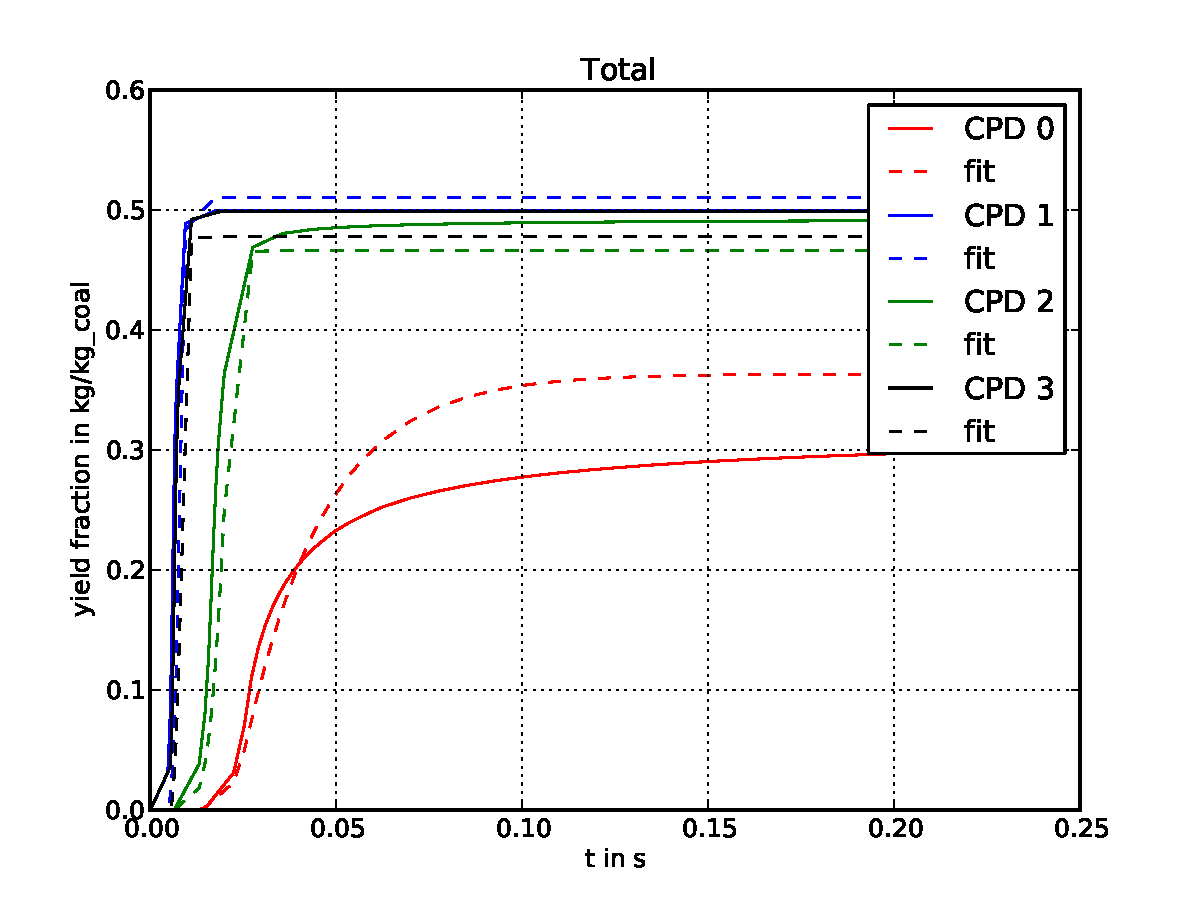
\includegraphics[height=9cm,angle=0]{Figures/CPD-Fit_result_Kob_Total_Y}
\caption{One fitting result (Yields) for the Kobayashi Model. The Kobayashi model just optimizes the overall yields.}
\label{F_Fit_Kob_Y}
\end{figure}

\begin{figure}
\centering%\capstart
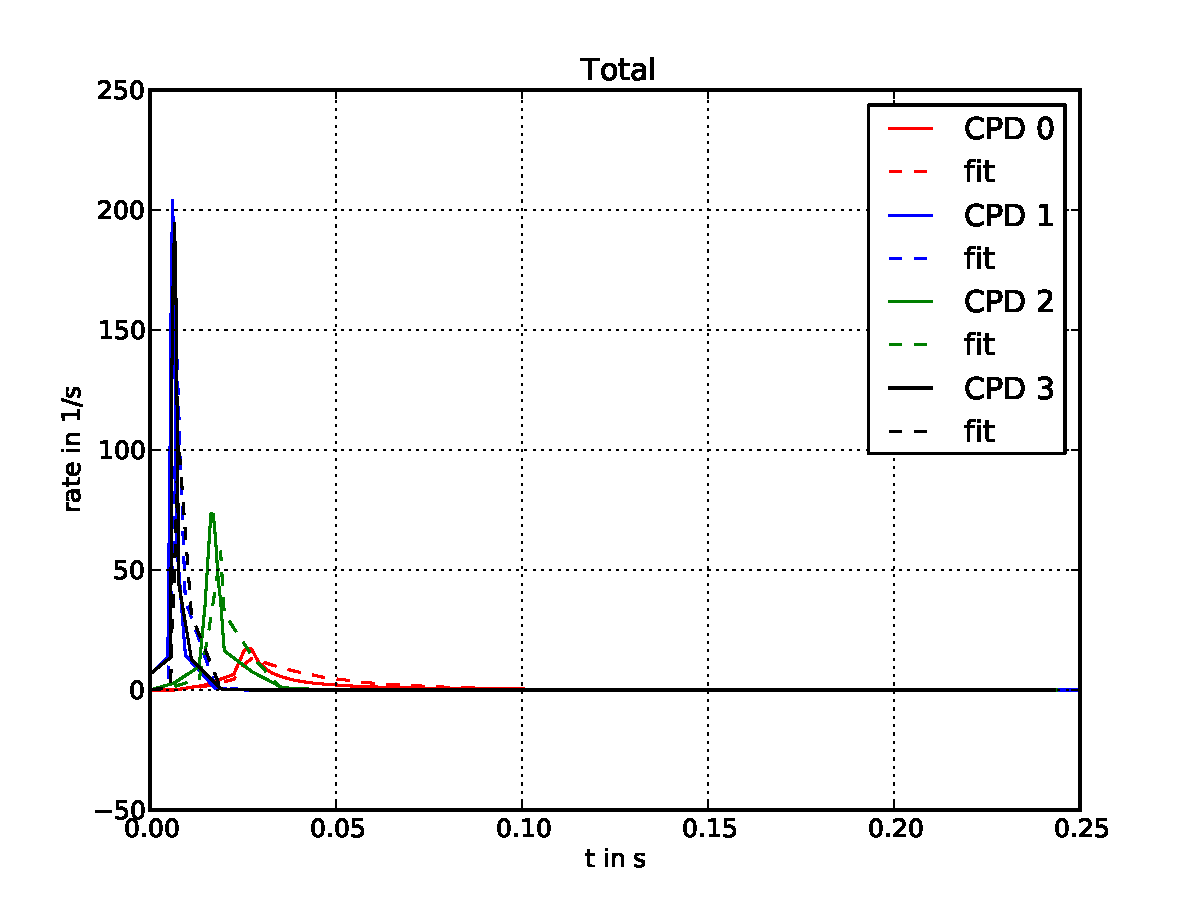
\includegraphics[height=9cm,angle=0]{Figures/CPD-Fit_result_Kob_Total_R}
\caption{One fitting result (Rates) for the Kobayashi Model.}
\label{F_Fit_Kob_R}
\end{figure}

\subsubsection{The Distributed Activation Energy Model}\label{SSS_DAEM}
The Distributed Activation Energy Model~(DAEM) considers parallel first order kinetics over a specific range, described by a distribution function~(F(E)). The equation used in PKP is:
\begin{equation}\label{E_DAEM}
 m = m_{final} \left( 1 - \int_{0}^{\infty} exp\left[ -A_0 \cdot \int^{t_{final}}_{t_0} exp\left( -\frac{E}{T} \right) dt  \right] F(E) \right)
\end{equation}
As a distribution function, a Gaussian Distribution is used:
\begin{equation}\label{E_GaussDistr}
 F(E) = \frac{1}{\sigma \cdot \sqrt{2\pi}} \cdot exp \left( -\frac{(E-E_0)^2}{2\sigma^2} \right)
\end{equation}
So there are four parameters to optimize:\\
\begin{enumerate}
 \item the preexponentiation factor $\mathrm{A_0}$, which is here equal for all reactions.
 \item $\mathrm{E_0}$, defining the center of the Gaussian Distribution
 \item and $\mathrm{\sigma}$, which spcifies the flattening of the Distribution curve and its range
 \item for multiple runs, the $\mathrm{m_{final}}$ also has to be optimized
\end{enumerate}
For solving the outer integral over dE, the Simpson tule is used. But for the nemuerical solution of the integral, the range has to be modified. As reported in the paper by Cai~\cite{Cai_DAEM1}, the integration boundaries can be se to $\mathrm{E_0 + 3 \cdot \sigma}$ as the upper and $\mathrm{E_0 - 3 \cdot \sigma}$ as the lower limit. This range covers up to 99.73~\% of the applied Gaussian Distribution. So for the further fitting of the devolatilization reaction, the prerequisite $\mathrm{E_0 > 3 \cdot \sigma}$ should be in force to achieve realistic results.\\
The inner integral $\mathrm{\int^{t_{final}}_{t_0} exp\left( -\frac{E}{T} \right) dt}$ was already simplyfied by setting $\mathrm{A_0}$ as a constant. In many papers~\cite{Cai_DAEM1,Cai_DAEM2,Cai_DAEM3,Slovak_DAEM} a linear heating rate over the whole time range is assumed, so $\mathrm{\frac{dT}{dt}=\beta}$. The transformation of the integral allows to integrate over the temperature. For such temperature integrals different analytical approaches exist~\cite{Cai_DAEM1,Cai_DAEM2}. This method was also tested.
 But as this is only a very specific case of the operating conditions and even not faster than solving the integrals\footnote{The reason might be that the very large analytical equations in Python (as an interpreting language) take more time than let the integral solve by a external library.}, this approach is furthernot considered. The double integral is solved numerically.\footnote{There are also other approaches to avoid the double integration like in the paper by McGuiness et al.~\cite{McGuiness_DAEM}, but also these assumptions made here ($\mathrm{\sigma \rightarrow 0 }$ or $\mathrm{\frac{E_0}{T} \rightarrow \infty }$) cannot be applied here.}\\
The outer integral is solved over a specific number of activation energies. For each activation energy the inner integral is solved and the value for all time steps saved, using a compisite Trapezoidal rule\footnote{the \texttt{scipy.integrate.cumtrapz} module, http://docs.scipy.org/doc/scipy/reference/generated/scipy.integrate.cumtrapz.html}. All inner integrals are saved in a 2D-Array($\mathrm{t_i,E_i}$). Each column contains all values of the inner integral for all time steps (the same activation energy), each line allinner integrals at the time $\mathrm{t_i}$. After this array is calculated, the equation of the outer integral is used for all values of the current line of the matrix and afterwards this list is integrated over dE.



\subsubsection{Fitting the Kinetic Equations}\label{SSS_FitKin}
The fitting procedure is carried out with a \texttt{scipy-optimizer}\footnote{\textit{http://docs.scipy.org/doc/scipy/reference/optimize.html}} \footnote{The standard setting optimizer is \texttt{fmin}.  The \texttt{leastsq} optimizer is the second choice.} and the \texttt{scipy.odeint}\footnote{\textit{http://docs.scipy.org/doc/scipy/reference/generated/scipy.integrate.odeint.html}} package to minimize the residual~$E(k,m_{fit})$ in the equation~\ref{E_LS}. For the structure of the whole fitting procedure see chapter~\ref{S_Program}. In equation~\ref{E_LS} is $\mathrm{m_{out}}$ the output of the devolatilization program \CPD or \FGDVC. The optimization is carried out over all points reported in the output file of the pyrolysis program. The normalized weight factor parameters~$\mathrm{a_0}$~and~$\mathrm{a_1}$ in the equations~\ref{E_Weight_Param1}~and~\ref{E_Weight_Param2} can both be defined by the user, the standard setting is for both one.

\begin{equation}\label{E_LS}
 E(k,m_{fit})=\omega_0 \int \left( m_{out}(t) - m_{fit}(k,t) \right)^2 dt \; + \; \omega_1 \int \left( \dot m_{out}(t) - \dot m_{fit}(k,t) \right)^2 dt
\end{equation}
\begin{align}
 \label{E_Weight_Param1}
\omega_0 &= \frac{a_0}{\left( max(m_{out})-min(m_{out}) \right)^2}\\
 \label{E_Weight_Param2}
\omega_1 &= \frac{a_1}{max(\dot{m}_{out}^2)}
\end{align}

\subsubsection{Pyrolysis Species- and Energy Conservation for \CPD output}\label{SSS_ConsEqCPD}

\paragraph{Species Conservation}
As the first step it has to be checked that the oxygen content in the generated yields~(oxygen containing species $\mathrm{f_i}$ with $\mu_i^{O}$ oxygen) is less equal that the oxygen in the ultimate analysis:
\begin{equation}
 UAO^{cpd, \: species \: output} = M_{O} \sum_i \frac{\mu_i^{O} f_i}{M_i} \le UAO 
 \label{E_O_balance}
\end{equation}
The factor~$\mathrm{\gamma}$~(\ref{E_gamma}) tells if the outputted yields contain less oxygen than reported in the Ultimate Analysis~(UA)~($\gamma > 1$) or if they are equal~($\gamma = 1$). For the case that~$\gamma < 1$, the oxygen containing yields have to be decreased by using equation~\ref{E_scale_up}, while the amount of the other species have to be increased to conserve the conserve the amount of volatile matter~(equation~\ref{E_add_up}). In this case, the tar will contain no oxygen. The yield of $N_2$ is equal to the UA of Nitrogen.

\begin{align}
 \gamma &= \frac{UAO}{UAO^{cpd, \: species \: output}}
 \label{E_gamma}\\
 f_i^{new} &= \gamma \cdot f_i 
 \label{E_scale_up}\\
 f_{oth}^{new} &= f_{oth} + \left(1-\gamma\right) \sum_i f_i
 \label{E_add_up}
\end{align}

For the case $f_{N_2}<f_{other}$, the remaining part is assigned to $CH_4$:

\begin{equation}
 f_{CH_4}^{new} = f_{CH_4} + \left( f_{oth}^{new} - f_{N_2} \right)
\label{E_MethanNew}
\end{equation}

Now the composition of tar can be calculated. For each element~C,H,O, the following equation~\ref{E_TarComp} can be used, assuming a tar composition of~$C_nH_mO_p$. $M_j$ is the atom weight of the element~j, $\mu_i^j$ the number of atoms of~$j$ in the species~$i$.

\begin{equation}
\frac{UA_j}{M_j} = \mu_{tar}^j \frac{f_{tar}}{M_{tar}} + \sum_i \mu_i^{j} \frac{f_{i}}{M_{i}}
%{UA_j} = \mu_{tar}^j \frac{f_{tar}}{M_{tar}} + \sum_i \mu_i^{j} \frac{f_{i}}{M_{i}}
\label{E_TarComp}
\end{equation}


\paragraph{Energy Conservation}
The Dulong formula is used, if the higher heating value~(HHV) of the coal is not known:
\begin{equation}\label{E_Dulong}
 HHV = 32.79 \cdot UAC + 150.4 \cdot (UAH - UAO/8) + 9.26 \cdot UAS + 4.97 \cdot UAO + 2.42 \cdot UAN
\end{equation}
where UAC, UAH, UAO, UAS and UAN are the value of the ultimate analysis for carbon, hydrogen, oxygen, sulfur and nitrogen. The result has the unit of~$\frac{MJ}{kg_{coal, as recieved}}$.\\

Afterwards, the HHV~(entered by the user or calculated with the Dulong formula) for the coal as received is related to the dry ash-free~(daf) state~(equation~\ref{E_HHVdaf}). This new HHV is used to get the lower heating value for a daf state, equation~\ref{E_LHV}. In this equation, $r_{H_2O}$ is the latent heat of water.
\begin{align}
 HHV_{daf}&=\frac{HHV_{ar}}{PAVM+PAFC}
\label{E_HHVdaf}\\
LHV_{daf}&=HHV_{daf}-\frac{M_{H_2O}}{2 \cdot M_H} \cdot UAH \cdot r_{H_2O}\
\label{E_LHV}
\end{align}

Regarding the combustion of the raw coal (equation~\ref{E_Raw_Comb}), the energy balance can be written as in equation~\ref{E_Raw_hf}.
\begin{align}
 &C_xH_y O_z N_w + (x + y/4 - z/2) O2 \rightarrow x CO2 + y/2 H2O + w/2 N2
\label{E_Raw_Comb}\\
&Q_{react}=LHV_{raw}\cdot M_{daf} = h_{f,raw} + (x + y/4 - z/2) h_{f,O_2} -x h_{f,CO_2} -y/2
	h_{f,H_2O} - w/2 h_{f,N_2}
\label{E_Raw_hf}
\end{align}
Using equation~\ref{E_Raw_hf}, the heat of formation of the raw molecule~($h_{f,raw}$) can be calculated.\\

The heat of formation for tar is based on the equation~\ref{E_DevolTar}, implying, that no heat is produced or absorbed during the devolatilization process.
\begin{equation}\label{E_DevolTar}
 C_x H_y O_z N_w \rightarrow \nu_{char}C_{(s)} + \nu_{tar} C_n H_m O_p + \sum_i \nu_i M_i
\end{equation}

The stoichiometric coefficient of each species can be calculated from the volatile yield expressed
as mass fraction:
\begin{equation}\label{E_myTar}
 \nu_i = \frac{f_i M_{raw}}{M_i}
\end{equation}
Making the energy balance for equation~\ref{E_DevolTar} with $Q_{react}=0$, the heat of formation for tar is:
\begin{equation}\label{E_Tar_hf}
 \nu_{tar} h_{f,tar} = h_{f,raw} - \nu_{char} h_{f,char} - \sum_i \nu_i h_{f,i}
\end{equation}\\

Another method is to assume a heat of formation for tar equal zero (e.g. if there is only a very low yield of tar), and calculate the heat of pyrolysis:
\begin{equation}
 - Q_{pyro} \cdot M_{raw} = h_{f,raw} - \nu_{char} h_{f,char} - \sum_i \nu_i h_{f,i}
\end{equation}
Where $Q_{pyro}$ is the heat of pyrolysis per unit of mass of daf. It is positive if heat is
required for breaking coal structure bounds. Generally, it is expressed in terms of volatile matter:
\begin{equation}\label{E_QPyro}
 Q_{pyro}^{vm} = \frac{Q_{pyro}}{1-f_{char}}
\end{equation}

\subsubsection{Pyrolysis Species and Energy Conservation for \FGDVC  output}\label{SSS_ConsEqFGDVC}
\paragraph{Species Conservation}
As in most of the CFD applications the combustion of some \FGDVC output species like HCN, COS or Olefins are not implemented. Only the species Char, Tar, CO, $CO_2$, $H_2O$, $CH_4$ and $H_2$ are further considered. The nitrogen is merged into the tar. So the amount of tar is calculated by the using equation~\ref{E_newTar}, where the sum contains the species Char, CO, $CO_2$, $H_2O$, $CH_4$ and $H_2$.
\begin{equation}\label{E_newTar}
 f_{Tar}=1-\sum_i f_i
\end{equation}
Applying the equation~\ref{E_TarComp} for all the elements~j~(Carbon, Hydrogen, Nitrogen, Oxygen), the composition of tar~(its stoichiometric coefficients) is calculated.\\

\paragraph{Energy Conservation}

Applying the energy balance on the combustion reaction of the devolatilization yields (for the case of a non-heat producing/consuming pyrolysis process), the following reaction equation is satisfied:
\begin{equation} \label{E_TarEnergy}
 LHV_{daf}=H_{f,Tar} \cdot f_{Tar} + \sum_i H_{f,i} \cdot f_{i}
\end{equation}
The LHV is calculated based on the HHV using the same equations as in chapter~\ref{SSS_ConsEqCPD}. The $H_{f,i}$ are calculated with the following equations~\ref{E_hf1}~to~\ref{E_hf4}, making an energy balance for every of the pyrolysis yields.
So the heat of formation for tar can be calculated from~equation~\ref{E_TarEnergy}, as all other parameters are known.

\begin{align}
\label{E_hf1}
 H_{f,Char}&=\left( (h_{f,Char}+h_{f,O_2}-h_{f,CO_2}) \cdot f_{Char} \right) \cdot M_C^{-1} \\
\label{E_hf2}
 H_{f,H_2}&=\left( (h_{f,H_2}+ \frac{1}{2} \cdot h_{f,O_2} - h_{f,H_2O}) \cdot f_{H_2} \right) \cdot M_{H_2O}^{-1} \\
\label{E_hf3}
 H_{f,CH_4}&=\left( (h_{f,CH_4}+ 2 \cdot h_{f,O_2}-h_{f,CO_2}-2 \cdot h_{f,H_2O}) \cdot f_{CH_4} \right) \cdot M_{CH_4}^{-1} \\
\label{E_hf4}
 H_{f,CO}&=\left( (h_{f,CO}+ \frac{1}{2} \cdot h_{f,O_2}-h_{f,CO_2}) \cdot f_{CO} \right) \cdot M_{CO}^{-1}
\end{align}

The $H_{f,Tar}$~with the unit~$\frac{J}{kg}$ is transformed back into~$\frac{J}{kmol}$ by multiplying with the molecular mass of tar.\\
To calculate the heat of formation for tar, the tar combustion can be regarded, as the tar composition is known:
\begin{equation}
 C_nH_mO_pN_k + \nu_{O_2} O_2 \rightarrow  \nu_{CO_2} CO_2 + \nu_{H_2O} H_2O + \nu_{N_2} N_2
\end{equation}

This leads to the balance, where the $h_{f,Tar}$ can be calculated:
\begin{equation}
 H_{f,Tar} = h_{f,Tar} + \nu_{O_2} h_{f,O_2} - \nu_{CO_2} h_{f,CO_2} - \nu_{H_2O} h_{f,H_2O} -\nu_{N_2} h_{f,N_2} 
\end{equation}

